\documentclass[a4paper]{standalone}

\usepackage{amsmath,stmaryrd}
\usepackage{tikz}
\usepackage{mathdots}
\usepackage{yhmath}
\usepackage{cancel}
\usepackage{color}
\usepackage{siunitx}
\usepackage{array}
\usepackage{multirow}
\usepackage{amssymb}
\usepackage{gensymb}
\usepackage{tabularx}
\usepackage{booktabs}
\usetikzlibrary{fadings}

\usepackage[T1]{fontenc}
\usepackage[utf8]{inputenc}

\usepackage{pgfplots}

\begin{document}


$ $


\tikzset{every picture/.style={line width=0.75pt}} %set default line width to 0.75pt        

% This file was created by tikzplotlib v0.9.1.
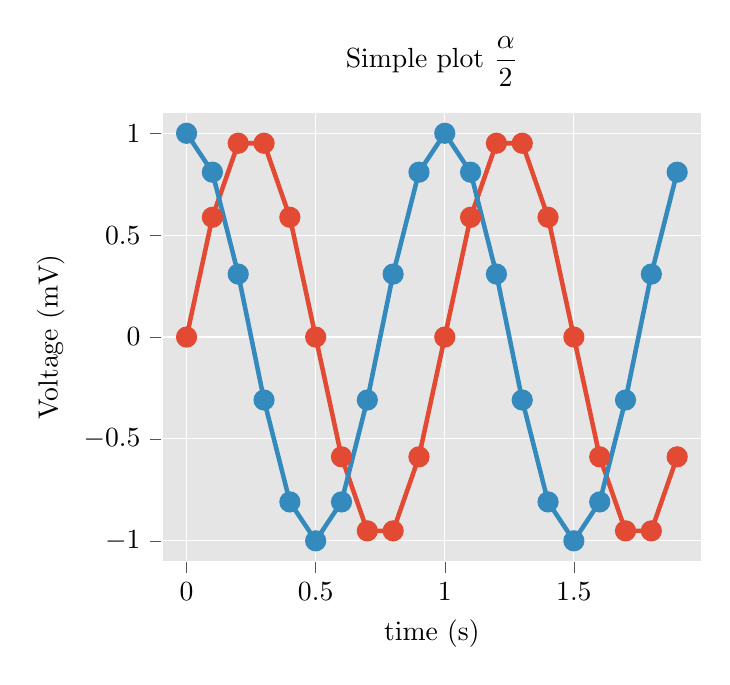
\begin{tikzpicture}

\definecolor{color0}{rgb}{0.886274509803922,0.290196078431373,0.2}
\definecolor{color1}{rgb}{0.203921568627451,0.541176470588235,0.741176470588235}

\begin{axis}[
axis background/.style={fill=white!89.8039215686275!black},
axis line style={white},
tick align=outside,
tick pos=left,
title={Simple plot \(\displaystyle \frac{\alpha}{2}\)},
x grid style={white},
xlabel={time (s)},
xmajorgrids,
xmin=-0.095, xmax=1.995,
xtick style={color=white!33.3333333333333!black},
y grid style={white},
ylabel={Voltage (mV)},
ymajorgrids,
ymin=-1.1, ymax=1.1,
ytick style={color=white!33.3333333333333!black}
]
\addplot [line width=1.64pt, color0, mark=*, mark size=3, mark options={solid}]
table {%
0 0
0.1 0.587785252292473
0.2 0.951056516295154
0.3 0.951056516295154
0.4 0.587785252292473
0.5 1.22464679914735e-16
0.6 -0.587785252292473
0.7 -0.951056516295154
0.8 -0.951056516295154
0.9 -0.587785252292473
1 -2.44929359829471e-16
1.1 0.587785252292474
1.2 0.951056516295154
1.3 0.951056516295154
1.4 0.587785252292473
1.5 3.67394039744206e-16
1.6 -0.587785252292473
1.7 -0.951056516295154
1.8 -0.951056516295154
1.9 -0.587785252292473
};
\addplot [line width=1.64pt, color1, mark=*, mark size=3, mark options={solid}]
table {%
0 1
0.1 0.809016994374947
0.2 0.309016994374947
0.3 -0.309016994374948
0.4 -0.809016994374947
0.5 -1
0.6 -0.809016994374947
0.7 -0.309016994374948
0.8 0.309016994374947
0.9 0.809016994374947
1 1
1.1 0.809016994374947
1.2 0.309016994374947
1.3 -0.309016994374947
1.4 -0.809016994374947
1.5 -1
1.6 -0.809016994374948
1.7 -0.309016994374946
1.8 0.309016994374947
1.9 0.809016994374947
};
\end{axis}

\end{tikzpicture}




\end{document}